\chapter{Blockchain Scalability}\label{ch:scalability}

\section{Bottlenecks in Scalability}
A blockchain's ability to scale is often measured by the amount of transactions it can verify per second. A block gets appended to the Ethereum blockchain every 12.5 seconds on average, and can contain only a finite amount of transactions. As a result, transaction throughput is bound by the frequency of new blocks and by the number of transactions in them.

We argue that there are two levels of scalability, scalability on contract and on network level. Better contract design can result in transactions which require less gas to execute, and thus allow for more transactions to fit in a block while also making it cheaper for the end user.With Ethereum's current blockGasLimit at 8003916, if all transactions in Ethereum were simple financial transactions\footnote{Not calls to smart contracts. Transactions without any extra data cost 21000 gas}, each block would be able to verify ~381 transactions, or 25 transactions per second (tps), which is still not comparable to traditional payment operators. 

\section{Network Level Scalability}
Scale should not be confused with scalability. While scale describes the size of a system and the amount of data being processed, scalability describes how the cost of running the system changes as scale increases. Existing blockchains scale poorly because the costs associated with them increase faster than the rate at which data can be processed. 

First of all, transactions per second as a metric is inaccurate. Solving scalability does not imply just increasing the transaction throughput. It is a constraint-satisfaction-problem; the goal is to maximize throughput while maintaining the network's decentralization and security. In the Ethereum Github, this is described as the \textit{Scalability Trilemma}.

\begin{quote}{Scalability Trilemma, Sharding FAQ}
    \textbf{This sounds like there’s some kind of scalability trilemma at play. What is this trilemma and can we break through it?}

    The trilemma claims that blockchain systems can only at most have two of the following three properties:

    \begin{itemize}
        \item Decentralization (defined as the system being able to run in a scenario where each participant only has access to $O(c)$ resources, ie. a regular laptop or small VPS)
        \item Scalability (defined as being able to process $O(n) > O(c)$ transactions)
        \item Security (defined as being secure against attackers with up to $O(n)$ resources)
    \end{itemize}
\end{quote}

An example that trades decentralization for more transactions is increasing the block size so that more transactions can fit inside a block and thus increase throughput. Increasing the size of each block, implies more disk space for storing the blockchain, better bandwith for propagating the blocks and more processing power on a node to verify any performed computations. This eventually requires computers with datacenter-level network connections and processing power which are not accessible to the average consumer, thus damaging decentralization which is the core value proposition of blockchain. % The blockGasLimit can be voted on by miners\footnote{\url{https://www.etherchain.org/tools/gasLimitVoting}}. % In addition to the reasons stated above, increasing the gas limit also potentially damages the security of the network due to increased uncle rates, Ethereum's analog to Bitcoin's orphan blocks \footnote{\url{https://blockchain.info/orphaned-blocks}}. Longer propagation time implies that a miner will spend more time searching for a solution until they receive a valid block, and thus has more chances of finding a valid block in that time. As a result, 

As described in \cite{scaling-trustless-models}, Proof of Work is a consensus algorithm optimized for censorship-resistance while (in theory) maintaining a low barrier to entry, as shown in Figure \ref{fig:scalability_triangle_pow}. Bitcoin and Ethereum's PoW networks have slow probabilistic time to finality and do not scale well. However, due to economies of scale, PoW blockchains end up being centralized around small numbers of miners \cite{Gencer2018DecentralizationIB}. 

\begin{figure}[ht!]
    \centering
    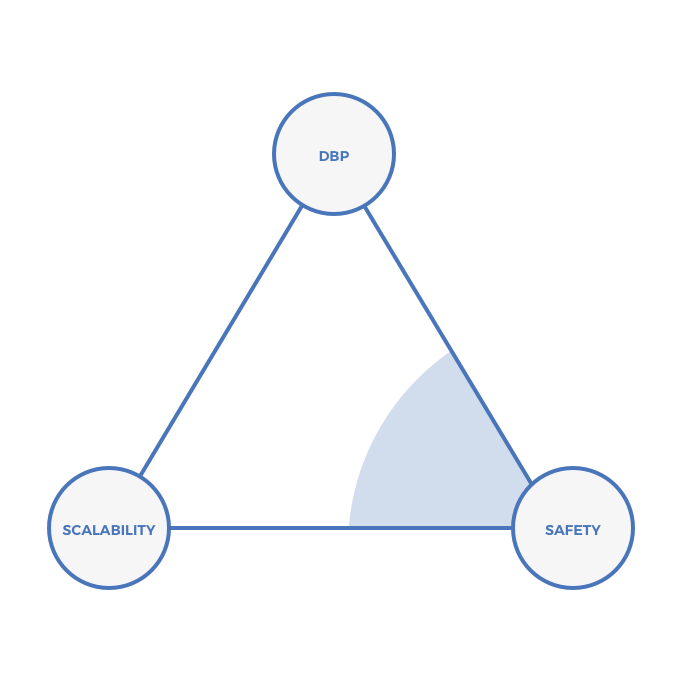
\includegraphics[width=0.5\textwidth]{scalability_triangle_pow}
    \caption{The Scalability Triangle~\cite{scaling-trustless-models}}
    \label{fig:scalability_triangle_pow}
\end{figure}

We proceed to discuss some network level solutions that can improve Ethereum's scalability.

\subsubsection*{Proof of Stake}
Proof of Stake (PoS) is an alternative consensus algorithm where in the place of miners, there are validators who instead of expending computational resources to `mine' a valid block, they stake\footnote{Lock up cryptocurrency for an amount of time and get paid in interest after a predefined time period.} their ether and the probability for them to be elected to validate the next block is proportional to their stake. Designing a secure PoS protocol is still under heavy research. The Ethereum Foundation is working on `Casper the Friendly Finality Gadget'~\cite{casperffg} which is a hybrid PoW/PoS consensus algorithm that provides block finality\footnote{A block that is finalized cannot be reverted. This is different to traditional PoW which achieves \textit{probabilistic finality}; a block is considered harder to revert the older it is.} which combined with the `correct-by-construction Casper the Friendly GHOST'\footnote{Uses the GHOST protocol to choose a chain in the case of a fork.} \cite{caspertfg} will enable a full transition to Proof of Stake. 

\subsubsection*{Sidechains}
A sidechain~\cite{sidechains} is a blockchain defined by a custom `rule-set' whihh cincbe used to offload computations from another chain. Individual sidechains can follow different sets of rules from the mainchain, which means they can optimize for applications that require high speeds or heavy computation, while still relying on the mainchain for issues requiring the highest levels of security. Ethereum's sidechain solution is called `Plasma' \cite{plasma} and involves creating \textit{Plasma chains} that run their own consensus algorithm and communicate with the mainchain via a two-way peg as described in \cite{sidechains}. \textit{Plasma chains} can have more adjustable parameters such as be less decentralized, however the protocol does not allow for the Plasma Chain operator to abuse their power. A more recent Plasma construct is called `Plasma-Cash' \cite{plasmacash} and describes a more efficient way of executing fraud proofs, in the case of a malicious actor in a \textit{Plasma chain}.

\subsubsection*{Sharding}
Due to the architecture of the EVM all transactions are executed sequentially on all nodes. Sharding~\cite{sharding} refers to splitting the process across nodes, so that each full node is responsible only for a shard\footnote{A shard is a part of the blockchain's state} and acts as a light client to the other shards. Sharding is the most complex scaling solution and is still at research stages. It also requires a stable Proof of Stake consensus algorithm to function properly.

\subsubsection*{State channels}
Contrary to the previous solutions which still record messages on a blockchain, state channels involves exchange of information `off-chain'. The primary use-case for state channels is micro-transactions between two or more parties. This technique involves exchanging signed messages through a secure communications channel and perform a transaction on the blockchain only when the process is done\footnote{Example: Instead of making 10 transactions worth 0.1 ether each, a transaction is made to open the channel, participants exchange off-chain messages transferring value, and settle or dispute the channel with one more transaction at the end.}.

\section{Contract Level Scalability}
In a recent study \cite{DBLP:journals/corr/ChenLLZ17}, after evaluating 4240 smart contracts, it is found that over 70\% of them cost more gas than they should due to the compiler failing to properly optimize the Solidity code during compilation. In this section we explore how gas gets computed in smart contracts and potential ways we can save on gas and transaction costs.

\subsection{Gas Costs}
An Ethereum transaction total gas costs are split in two: % https://ethereum.stackexchange.com/a/29560
\begin{enumerate}
    \item \textbf{Base Transaction Costs:} The cost of sending data to the blockchain. There are 4 items which make up the full transaction cost:
        \begin{enumerate}
            \item The base cost for a transaction (21000 gas). % hereafter gas units will be referred to as gas
            \item Extra cost in the case that the transaction involves deploying a contract (32000 gas).
            \item The cost for every zero byte of data in the transaction input field (4 gas per zero byte).
            \item The cost of every non-zero byte of data in the transaction input field (68 gas per non-zero byte).
        \end{enumerate}
    \item \textbf{Execution Costs:} The cost of computational operations which are executed as a result of the the transaction, as described in detail in \cite{ethereum, gas}.
\end{enumerate} 

Gas costs get translated to transaction fees. As a result, a contract should be designed to minimize its operational gas costs in order to minimize its transaction fees. Transactions that cost less gas allow more room for other transactions to be included in a block which can improve scalability. % In addition, as gas is a unit for computational costs, less gas consumed results in less burden on the nodes validating the smart contracts which can lead to better scalability.

\begin{table}[H]
	\centering
	\vspace*{-1ex}
	\scriptsize
	\caption{Gas cost of different operations, a complete list can be found in Ethereum's yellow paper~\cite{gas}, from \cite{DBLP:journals/corr/ChenLLZ17}}
	\vspace{-1ex}
	\label{table:opcode_table}
	\begin{tabular}{|c|c|c|}
		\hline
		\textbf{Operation}        & \textbf{Gas} & \textbf{Description} \\ \hline
		\textsc{ADD/SUB}          & 3 & \multirow{3}{*}{Arithmetic operation} \\ \cline{1-2}
		\textsc{MUL/DIV}          & 5 & \\ \cline{1-2}
		\textsc{ADDMOD/MULMOD}    & 8 & \\ \hline
		\textsc{AND/OR/XOR}       & 3 & Bitwise logic operation \\ \hline
		\textsc{LT/GT/SLT/SGT/EQ} & 3 & Comparison operation \\ \hline
		\textsc{POP}              & 2 & \multirow{2}{*}{Stack operation} \\ \cline{1-2}
		\textsc{PUSH/DUP/SWAP}    & 3 & \\ \hline
		\textsc{MLOAD/MSTORE}     & 3 & Memory operation \\ \hline
		\textsc{JUMP}             & 8 & Unconditional jump \\ \hline
		\textsc{JUMPI}            & 10 & Conditional jump \\ \hline
		\textsc{SLOAD}            & 200 & \multirow{2}{*}{Storage operation} \\ \cline{1-2}
		\textsc{SSTORE}           & 5,000/20,000 & \\ \hline
		\textsc{BALANCE}          & 400 & Get balance of an account \\ \hline
		\textsc{CREATE}           & 32,000 & Create a new account using CREATE \\ \hline
		\textsc{CALL}             & 25,000 & Create a new account using CALL \\  \hline
	\end{tabular}
	\vspace{-2ex}
\end{table}

% bytecontracts includes constructor and general initialisation contracts which is not needed anymore at runtime. The contracts that is sent during deployment (bytecontracts), even excluding the constructor arguments, is - in general - different from the contracts that is stored at that address (the runtimeBytecontracts).

As seen in Table \ref{table:opcode_table}, the most expensive operations involve CREATE\footnote{Used to create a new contract.} and SSTORE\footnote{Used to store data operations}. The focus of this section will be to explore ways to decrease gas costs on Smart Contracts, either through better practices or by handcrafting optimizations for specific use cases.

It should be noted, that non-standard methods have been proposed for reducing fees incurred by gas costs. A recent construction \cite{gastoken} describes a method of buying gas at low cost periods and saving it in order to spend it when gas prices are higher\footnote{When the network is congested}. The economic implications of gas arbitrage are outside the scope of this Master Thesis. 

General rules that should be followed for saving gas costs:
\begin{enumerate}
    \item Enable compiler optimizations (although this has lead to unexpected scenarios~\cite{compiler}).
    \item Reuse code through libraries~\cite{library}.
    \item Setting a variable back to zero refunds 15000 gas through SSTORE, so if a variable is going to be unused it is considered good practice to call \texttt{delete} on it. 
    \item When iterating through an array, if the break condition involves the array's length set it as a stack variable the loop. This way, it doesn't get loaded during each loop and allows for saving 200 gas per iteration \cite{DBLP:journals/corr/ChenLLZ17}.
    \item Use \texttt{bytes32} instead of \texttt{string} for strings that are of known size. \texttt{bytes32} always fit in an EVM word, while \texttt{string} types can be arbitrarily long and thus require more gas for saving their length.
    \item Do not store large amounts of data on a blockchain. It is more efficient to store a hash which can be either proof of the existence of the data at a point in time, or it can be a hash pointing to the full data\footnote{This pattern has been used in combination with IPFS, \url{https://ipfs.io}}.
\end{enumerate}

As described in \cite{DBLP:journals/corr/ChenLLZ17} there is a lot of room for further compiler optimizations. Future Solidity compiler versions are addressing some already\footnote{\url{https://github.com/ethereum/solidity/issues/3760}}\footnote{\url{https://github.com/ethereum/solidity/issues/3716}}\footnote{\url{https://github.com/ethereum/solidity/issues/3691}}.

The EVM operates on 32 byte (256 bit) words. The compiler is able to `tightly pack' data together, which means that 2 128 bit storage variables can be efficiently stored with 1 SSTORE command. The \textit{optimize} flag of the Solidity compiler needs to be activated to access this feature when programming in Solidity. Refer to \ref{fig:struct_optimization} for an example of the optimizer's functionality.

\subsection{Gas Savings Case Study}

We proceed to compare the gas efficiency of 3 methods for storing data in a smart contract based on a gaming use-case. The contract design requirements are: 
\begin{itemize}
    \item A user must be able to register as a player in the contract.
    \item A player must be able to create a character with certain traits as function arguments.
    \item A player must be able to retrieve the traits of a character.
\end{itemize}

\begin{table}[H]
	\centering
	\vspace*{-1ex}
	\scriptsize
	\vspace{-1ex}
	\begin{tabular}{|c|c|c|}
        \hline
        \textbf{Name} & \textbf{Type}  & \textbf{Comment}\\ \hline 
        playerID      & uint16         & Game supports up to 65535 players\\
        creationTime  & uint32         & Game supports timestamps up to 2**32 = 02/07/2106 @ 6:28am (UTC) \\
        class         & uint4          & Game supports up to 16 classes \\
        race          & uint4          & Game supports up to 16 classes \\
        strength      & uint16         & Stats can be up to 65535\\
        agility       & uint16         & Stats can be up to 65535 \\
        wisdom        & uint16         & Stats can be up to 65535 \\
        metadata      & bytes18        & Utilize the rest of the word for metadata \\
        \hline
    \end{tabular}
	\caption{Required variables and size. Sizes add up to 248 bits which can be efficiently stored in a 256 bit word.}
    \label{table:characteristics}
\end{table}


The choice of variables in Table \ref{table:characteristics} is made to represent what the traits of a character would be in a game built on a smart contract. The size of the variables is selected so that all the information required to describe a \texttt{Character} can fit in a 256 bit word. The interface that satisfies the requirements is shown in~\ref{fig:game_interface}.

We will examine the gas costs for deployment and for calling each function for the following implementations:

\begin{enumerate}
    \item Packing of traits by utilizing Solidity's optimizer and \texttt{struct} variables
    \item Manually pack traits in a \texttt{uint256} variable with masking and shifting.
    \item Manually pack traits in a \texttt{bytes32} variable (equivalent in length to \texttt{uint256}) with masking and shifting, utilizing Solidity Libraries, influenced by~\cite{virtualstruct}.
\end{enumerate}
We use \texttt{bytes32} in Method 3 because the bit operations done in Solidity when extracted in functions do not function as expected with \texttt{uint256} variables. The full contract implementations for each method can be found in Appendix \ref{apx:scalability}. A comparison of the performance for each method is shown in \ref{ch:scalability:results}% In this section we describe the methods and in section \label{results} we go over the results and caveats of each method.

\subsubsection{Packing of traits by utilizing Solidity's optimizer and \texttt{struct} variables} \label{method1}
We use Solidity's built-in \texttt{struct}\footnote{\url{http://solidity.readthedocs.io/en/v0.4.21/types.html}} keyword as means to group all traits of a \texttt{Character} as described in \ref{table:characteristics}. This allows for easy code readability since every variable of a \texttt{struct} can be accessed by its name as seen in \ref{fig:struct_optimization:c}, like the property of an object. 

\begin{figure}[ht!]
    \begin{subfigure}[b]{\textwidth}
        \centering
        \lstinputlisting[language=Solidity, firstline=1, lastline=9]{contracts/CreateCharacter.sol}
        \caption{Method 1: \texttt{CreateCharacter}}
        \label{fig:method1:createcharacter}
    \end{subfigure}

    \begin{subfigure}[b]{\textwidth}
        \centering
        \lstinputlisting[language=Solidity, firstline=29, lastline=39]{contracts/CreateCharacter.sol}
        \caption{Method 1: \texttt{GetCharacterStats}}
        \label{fig:method1:getcharacterstats}
    \end{subfigure}
    \caption{Method 1 API}
    \label{fig:method1}
\end{figure}

In this case, assignment and retrieval of the variables is done in a very straightforward way. By utilizing Solidity's built-in structures and arrays, we can create an array of \texttt{Character} type structures and access their traits by their indexes, as done in \ref{fig:struct_optimization:c}. The gas costs per function call with this method are shown in \ref{table:tightpacking}.

\begin{table}[H]
	\centering
	\caption{Gas costs for deployment and for each function using Solidity's built-in structs}
	\vspace*{-1ex}
	\scriptsize
	\vspace{-1ex}
	\begin{tabular}{|c|c|c|c|}
		\hline
		\textbf{Optimizer Runs} & \textbf{Register} & \textbf{CreateCharacter} & \textbf{Deployment} \\ \hline
        0      &    70003 &          104205 &    903173.0 \\
        1      &    69943 &          104202 &    529979.0 \\
        100    &    69811 &          103402 &    561342.0 \\
        500    &    69604 &          103207 &    586867.0 \\
		500000 &    69598 &          103183 &    651665.0 \\
		\hline
    \end{tabular}
	\vspace{-2ex}
	\label{table:tightpacking}
\end{table}

\subsubsection{Manually pack traits in a uint256 variable with masking and shifting} \label{method2}
    
In \ref{method1} we rely on the optimizer to make storing a character's traits more efficient. It turns out\footnote{\url{https://github.com/figs999/Ethereum/blob/master/Solc.aComedyInOneAct}} that the optimizer is not able to remove all unnecessary operations and there is still room for improvement. In order to get better results, we create a local stack variable\footnote{The data is 248 bits long, so we create a \texttt{uint256} variable} which is large enough to store all the traits from \ref{table:characteristics}. Instead of creating a \texttt{struct}, we manually encode each trait in the said variable, essentially we act as the optimizer, which results in much less gas spent as both the contract's bytecode is smaller and the \texttt{CreateCharacter} function is more efficient. We proceed to describe the encoding process.

\begin{figure}[ht!]
    \makebox[\linewidth][c]{%
    \begin{subfigure}[b]{0.5\textwidth}
        \centering
        \lstinputlisting[language=Solidity, firstline=11, lastline=18]{contracts/CreateCharacter.sol}
        \caption{Method 2: \texttt{CreateCharacter}}
        \label{fig:method2:createcharacter}
    \end{subfigure}

    \hspace{1cm}

    \begin{subfigure}[b]{0.58\textwidth}
        \centering
        \lstinputlisting[language=Solidity, firstline=41, lastline=50]{contracts/CreateCharacter.sol}
        \caption{Method 2: \texttt{GetCharacterStats}}
        \label{fig:method2:getcharacterstats}
    \end{subfigure}
    }
    \caption{Method 2 API}
    \label{fig:method2}

\end{figure}

% By left shifting a trait's value by the sum of the size of all variables to its right and then performing a bitwise OR operation with the \texttt{uint256}, the trait gets encoded in the \texttt{uint256}, as shown in~\ref{fig:uint_encoding}. 

Setting data requires shifting left $N$ times and performing bitwise OR with the target variable, where $N$ is the sum of the number of bits of all variables to the right of the target variable, as shown in Figure \ref{fig:uint_encoding}. This is implemented in \ref{fig:uint_encoding_code}

\begin{figure}[H]
    \centering
    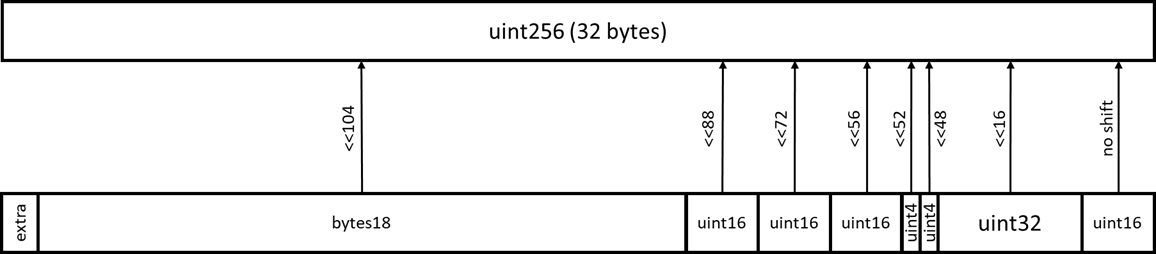
\includegraphics[width=\textwidth]{uint_encoding}
    \caption{Encoding data in a \texttt{uint256} variable}
    \label{fig:uint_encoding}
\end{figure}

% By right shifting the \texttt{uint256} by the sum of the size of all variables to the right of a trait and then performing a bitwise AND operations with the trait's size retrieves the value of the trait. 

Retrieving data requires shifting right $N$ times and performing bitwise AND with the target variable's size, where $N$ is the sum of the number of bits of all variables to the right of the target variable. Figure \ref{fig:uint_decoding} illustrates retrieving the \texttt{creationTime} trait from the \texttt{uint256} by shifting right 16 times and performing bitwise AND with $2^{32}-1$ since \texttt{creationTime} is a 32 bit variable. This is implemented in \ref{fig:uint_decoding_code}.

\begin{figure}[H]
    \centering
    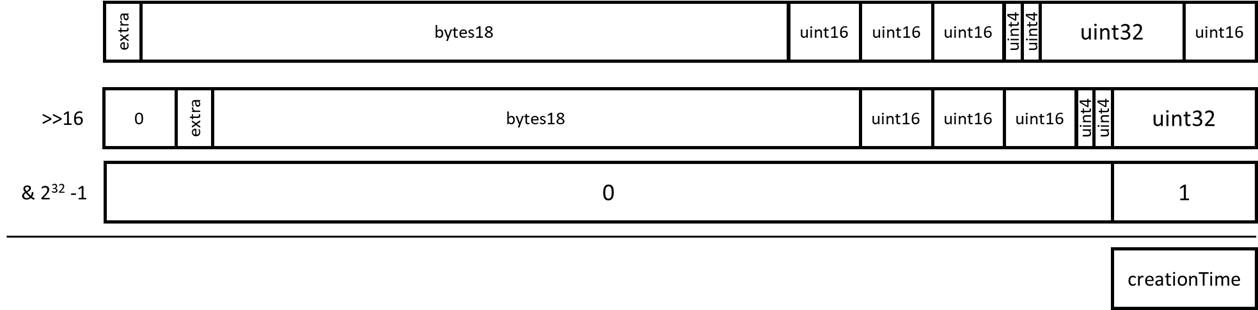
\includegraphics[width=\textwidth]{uint_decoding}
    \caption{Retrieving \texttt{creationTime} from the encoded \texttt{uint256}}
    \label{fig:uint_decoding}
\end{figure}

The gas costs per function call with this method are: 
\begin{table}[H]
	\centering
	\caption{Gas costs for deployment and for each function using the masking method on a uint.}
	\vspace*{-1ex}
	\scriptsize
	\vspace{-1ex}
	\begin{tabular}{|c|c|c|c|}
		\hline
		\textbf{Optimizer Runs} & \textbf{Register} & \textbf{CreateCharacter} & \textbf{Deployment} \\ \hline
        0      &    70003 &           66620 &    551800.0 \\
        1      &    69943 &           66365 &    378022.0 \\
        100    &    69811 &           65924 &    402120.0 \\
        500    &    69604 &           65855 &    419559.0 \\
		500000 &    69598 &           65855 &    432409.0 \\
		\hline
	\end{tabular}
	\vspace{-2ex}
	\label{table:uint_masking_gas}
\end{table}

\subsubsection{Manually pack traits in a bytes32 variable with masking and shifting, utilizing Solidity Libraries} \label{method3}

Code reusability and readability should always be given high priority. Although data packing is very efficient in~\ref{method2} compared to~\ref{method1}, the code is hardly readable and it is impossible to reuse parts of it. % It is possible to extract the logic into functions, however the overheads introduced by the additional operations make it inferior to the technique we describe in this section.
We utilize Solidity's \texttt{Library} built-in which allows us to define a set of methods which can be applied on a datatype using the \texttt{using X for Y} syntax\footnote{This is similar to calling functions on struct's in Golang}. A simple example is shown in \ref{fig:library}.


The visibility of a Library's exported functions can be: 
\begin{enumerate}
    \item \textbf{Internal:}
        In this case, the compiled library's bytecode is inlined to the main contract's code. This results in larger bytecode during deployment, however each of the Library's functions are called via the \texttt{JUMP} opcode. In this case, only the base contract needs to be deployed.
    \item \textbf{Public:}
        In this case, the main contract's bytecode has placeholder slots. These slots get filled by the Library's address which is obtained after deploying the Library contract. After replacing the placeholder slots with the Library's address, any function call to the library is done via the \texttt{DELEGATECALL} opcode.
\end{enumerate}

% Should insert placeholder and inlined bytecode? 

Libraries with public functions are deployed as standalone contracts to be used by contracts made by other developers. This process is further described in \ref{apx:scalability:lib}. They often include generic functionality such as math operations\footnote{A popular Solidity Library is \texttt{SafeMath} which contains error-checked math operations}. Depending on the complexity of the contracts, this can be more efficient compared to using \texttt{internal} functions. % When \textit{public} is used, the DELEGATECALL opcode is used\footnote{Relays the message to the library while allowing it to execute in the sender's state}. When \textit{internal} is used, a function call is interpreted as a jump and thus is more efficient than the DELEGATECALL. 

The final version is split in two files, the library which includes the API for setting and retrieving the character's traits, and the main contract which uses the library's high-level functions. By utilizing the \texttt{using CharacterLib for bytes32} syntax we are able to store and retrieve a character's traits in a user-friendly manner.

\begin{figure}[ht!]
    \begin{subfigure}[b]{\textwidth}
        \centering
        \lstinputlisting[language=Solidity, firstline=20, lastline=27]{contracts/CreateCharacter.sol}
        \caption{Method 3: \texttt{CreateCharacter}}
        \label{fig:method3:createcharacter}
    \end{subfigure}

    \begin{subfigure}[b]{\textwidth}
        \centering
        \lstinputlisting[language=Solidity, firstline=52, lastline=62]{contracts/CreateCharacter.sol}
        \caption{Method 3: \texttt{GetCharacterStats}}
        \label{fig:method3:getcharacterstats}
    \end{subfigure}
    \caption{Method 3 API}
    \label{fig:method3}

\end{figure}
That way, instead of having to deploy a new contract, developers can use an already deployed one. Due to the usage of \texttt{DELEGATECALL}, there is a tradeoff between contract deployment costs and the extra costs incurred when making function calls. We use \texttt{internal} because it requires less gas and since this is a specialized use-case it is not expected to be used by third-parties.

The gas costs per function call with this method are: 
\begin{table}[H]
	\centering
	\vspace*{-1ex}
	\scriptsize
	\vspace{-1ex}
	\label{table:byte_masking_gas}
	\begin{tabular}{|c|c|c|c|}
		\hline
		\textbf{Optimizer Runs} & \textbf{Register} & \textbf{CreateCharacter} & \textbf{Deployment} \\ \hline
        0      &    70003 &           67581 &    754613.0 \\
        1      &    69943 &           67414 &    508014.0 \\
        100    &    69811 &           66904 &    538621.0 \\
        500    &    69604 &           66835 &    556054.0 \\
		500000 &    69598 &           66835 &    569032.0 \\
		\hline
    \end{tabular}
	\vspace{-2ex}
	\caption{Gas costs for deployment and for each function using the masking method on bytes32 utilizing Libraries.}
\end{table}

\subsection{Results}\label{ch:scalability:results}
Observing \ref{table:tightpacking}, \ref{table:uint_masking_gas} and \ref{table:byte_masking_gas},  it is seen that in all cases the optimizer's first iteration creates significant gas savings. Further optimizer runs result in more gas expenditure during deployment but less per function call. This happens because \texttt{solc} optimizes either for size or for runtime costs\cite{optimizer-tradeoff}. In this section we compare the gas costs for calling the \texttt{CreateCharacter} function and for deploying the contract for 1 optimizer run\footnote{We do not compare \texttt{Register} because the implementation is the same across all 3 methods and \texttt{GetCharacterStats} does not cost gas to call externally because it is a \texttt{view} method which does not modify the state.}. 

\begin{figure}[ht!]
    \makebox[\linewidth][c]{%
    \begin{subfigure}[c]{0.58\textwidth}
        \centering
        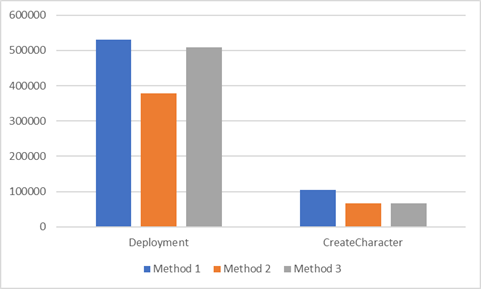
\includegraphics[width=\textwidth]{comparison_methods}
        \label{fig:gascomp:absolute}
    \end{subfigure}

    \hspace{1cm}

    \begin{subfigure}[c]{0.58\textwidth}
        \centering
        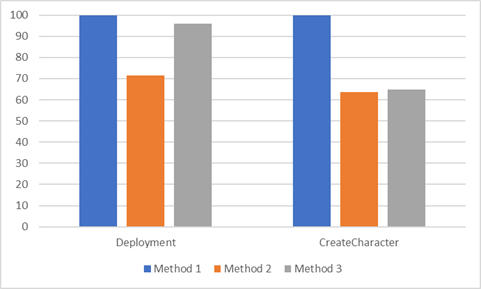
\includegraphics[width=\textwidth]{comparison_methods_pct}
        \label{fig:gascomp:pct}
    \end{subfigure}
    }
    \caption{Gas cost comparison between the 3 proposed methods.}
    \label{fig:gascomp}
\end{figure}

It is clear that the biggest savings are achieved through Method 2. Deploying a contract with Method 2 is 29\% more efficient than Method 1, while Method 3 is only 4\% more efficient than Method 1. Calling \texttt{CreateCharacter} is approximately 36\% more efficient in both methods compared to Method 1. 

Method 2 is the most efficient in terms of gas, however the coding style used for it is extremely compact and non-verbose, which makes difficult to maintain and modify the code, in case software requirements change, as seen in \ref{fig:method2}. In addition, there is no measure taken for overflows, so in case the \texttt{CreateCharacter} function gets called with an argument that is larger than the designed size, the result is miscalculated (\ref{apx:scalability:overflow}) 

In an attempt to improve the readability and maintainability of the method by extracting the bit shifting logic to functions the deployment gains over Method 3 are in the range of 5\%, and the function costs differ in the range of 0.001\%, thus negating most of the gas efficiency advantages.


On the other hand, by comparing Method 1 (Figure \ref{fig:method1}) with Method 3 (Figure \ref{fig:method3}) it is seen that they have very similar syntax, with Method 1 being much more efficient in terms of gas. In addition, the bit shifting logic is extracted to a library which makes the code fully portable. Finally, there is more flexibility when performing bit operations due to the usage of \texttt{bytes32} in the library and as a result there is no risk of variables overflowing, contrary to Method 2.

% similar gas efficiency when it comes to calling \texttt{CreateCharacter}. The increased deployment costs happen because it utilizes the \texttt{CharacterLib}, described in \ref{apx:scalability:lib}


In order to effectively compare and evaluate which method is the most effective for the described use case, we evaluate on a weighted score based on \textit{Readability}, \textit{Portability}, \textit{Gas Efficiency} and \textit{Security}, as illustrated in Table \ref{table:weights}.

\begin{table}[H]
	\centering
	\vspace*{-1ex}
	\caption{Selected weights for evaluation criteria.} 
	\scriptsize
	\vspace{-1ex}
	\begin{tabular}{|c|c|c|}
        \hline
        \textbf{Name} & \textbf{Weight}  & \textbf{Description}\\ \hline 
        \textbf{Readability} & 0.25 & How readable is the code\\
        \textbf{Portability} & 0.2 & How easy is it to use the code in another smart contract? \\
        \textbf{Gas Efficiency} & 0.3 & How gas efficient is the code? \\
        \textbf{Security} & 0.25 & How robust and secure is the code? \\
        \hline
    \end{tabular}
    \label{table:weights}
\end{table}


Taking the above into consideration, we choose to use Method 3 in order to make the implementation described in Chapter \ref{ch:implementation} more gas efficient while retaining its readability and maintainability. The results of the evaluation are shown in Table \ref{table:evaluation}:

\begin{table}[H]
	\centering
	\caption{Evaluation of each method}
	\vspace*{-1ex}
	\scriptsize
	\vspace{-1ex}
	\begin{tabular}{|c|c|c|c|c|c|c|c|c|}
        \hline
        \textbf{Name} & \textbf{Weight}  
      & \textbf{M1} & \textbf{M1 (W)}
      & \textbf{M2} & \textbf{M2 (W)} 
      & \textbf{M3} & \textbf{M3 (W)}\\ 
        \hline 
        \textbf{Readability/Maintainability} 
            & 0.25 & 5  & 1.25 & 3 & 0.75 & 4 & 1\\
        \textbf{Portability} 
            & 0.2  & 5  & 0.8  & 3 & 0.6  & 4 & 0.8\\
        \textbf{Gas Efficiency} 
            & 0.3  & 1  & 0.3  & 5 & 1.5  & 4 & 1.2\\
        \textbf{Security} 
            & 0.25 & 5  & 1.25 & 4 & 1    & 4 & 1\\
        \hline
        \textbf{Total} 
            & 1    & 16 & 3.8  & 15 & 3.85 & 16 & 4\\
        \hline
    \end{tabular}
    \label{table:evaluation}
\end{table}


% In Method 1 (\ref{table:tightpacking}) the optimizer is able to cut down deployment costs by 42\%, due to being able to pack all variables in a storage slot. 

% In Method 2 (\ref{table:uint_masking_gas}), the optimization is done manually and has significant results both in deployment and in function costs. In Method 3 (\ref{table:byte_masking_gas}), although we follow the same pattern as in Method 2, we introduce a more verbose API which results in more complex operations being done at a lower level. This introduces slightly bigger deployment costs, and a negligible difference in gas costs for function calls. We consider this overhead to be worth it, since we export an API that is usable.

% Deciding how many times to run the optimizer requires estimating the expected usage of the smart contracts. Comparing the results from running the optimizer 1 and 500 times in Method 2, it can be seen that the deployment costs can increase by as much as 10\% while the savings for each function call are in the range of 0.7\%. When quantifying these percentages in gas, we conclude that if a function is going to be called \textit{enough}\footnote{Enough is not quantifiable and depends on the implementation. A developer should perform a similar analysis to the one we do in order to set their breakeven points.} times, then the contract which was compiled with more optimizer runs is more efficient in the long run. In addition, this shifts the costs towards the contract deployer rather than the users. Given the tradeoffs described above and the improved code readability and maintainability, we opt to use Method 3 in our implementations. 

% Depending on how many times the optimizer is run, there is a different breakeven point for making it worth running more than one times. Running the optimizer 100 times requires the `CreateCharacter' function to be called at least 24 times to make it worth it. % EXPLAIN BETTER THE QUANTIFICATION OF THE TRADEOFF PER FUNCTION CALL COMPARED TO DEPLOYMENT COSTS. Also, the initial cost comes on deployment from the deployer side 
% Even though 1300 gas at the price of 20gwei translates to 0.0000299 https://ethgasstation.info/calculatorTxV.php, this can be a considerable amount considering that a funciton call in a decentralized future might be called millions of times. 1 

% In addition, as we essentially do the optimization ourselves, the deployed bytecode is smaller. 
% This is not exactly intuitive, as it'd be expected that the solidity compiler is able to pack everything perfectly. this method is far more efficient. With this method we are able to store and fetch all the data in a very efficient way, which costs X\% gas less than the previous implementation. However, this method does not allow for a readable and maintainable interface. In order to export every functionality it is needed to convert the `uint' variables to bytes to perform the bit operations on functions. This creates undesired overhead and thus is avoided.

%We described a technique which relies on the compiler's optimizer to pack the data in a struct and do the gas savings, however is simpler and more elegant. The second and third technique are more complex and allow for further gas optimizations. The second technique is more efficient however lacks reusability and is less maintaneable. On the other hand, utilizing libraries however we can export a user-friendly API for reusing our code for anyone who has the same use case as us. This technique will be utilized in the Design and implementation section.